\documentclass[11pt]{article} 
\usepackage[english]{babel}
\usepackage[utf8]{inputenc}
\usepackage[margin=0.5in]{geometry}
\usepackage{amsmath}
\usepackage{amsthm}
\usepackage{amsfonts}
\usepackage{amssymb}
\usepackage[usenames,dvipsnames]{xcolor}
\usepackage{graphicx}
\usepackage[siunitx]{circuitikz}
\usepackage{tikz}
\usepackage[colorinlistoftodos, color=orange!50]{todonotes}
\usepackage{hyperref}
\usepackage[numbers, square]{natbib}
\usepackage{fancybox}
\usepackage{epsfig}
\usepackage{soul}
\usepackage[framemethod=tikz]{mdframed}
\usepackage[shortlabels]{enumitem}
\usepackage[version=4]{mhchem}
\usepackage{multicol}
 
\usepackage{mathtools}
\usepackage{comment}
\usepackage{enumitem}
\usepackage[utf8]{inputenc}
\usepackage[linesnumbered,ruled,vlined]{algorithm2e}
\usepackage{listings}
\usepackage{color}
\usepackage[numbers]{natbib}
\usepackage{subfiles}
\usepackage{tkz-berge}


\newtheorem{prop}{Proposition}[section]
\newtheorem{thm}{Theorem}[section]
\newtheorem{lemma}{Lemma}[section]
\newtheorem{cor}{Corollary}[prop]

\theoremstyle{definition}
\newtheorem{definition}{Definition}

\theoremstyle{definition}
\newtheorem{required}{Problem}

\theoremstyle{definition}
\newtheorem{ex}{Example}


\setlength{\marginparwidth}{3.4cm}
%#########################################################

%To use symbols for footnotes
\renewcommand*{\thefootnote}{\fnsymbol{footnote}}
%To change footnotes back to numbers uncomment the following line
%\renewcommand*{\thefootnote}{\arabic{footnote}}

% Enable this command to adjust line spacing for inline math equations.
% \everymath{\displaystyle}

% _______ _____ _______ _      ______ 
%|__   __|_   _|__   __| |    |  ____|
%   | |    | |    | |  | |    | |__   
%   | |    | |    | |  | |    |  __|  
%   | |   _| |_   | |  | |____| |____ 
%   |_|  |_____|  |_|  |______|______|
%%%%%%%%%%%%%%%%%%%%%%%%%%%%%%%%%%%%%%%

\title{
\normalfont \normalsize 
\textsc{CSCI 3104 Spring 2022 \\ 
Instructors: Profs. Chen and Layer} \\
[10pt] 
\rule{\linewidth}{0.5pt} \\[6pt] 
\huge Quiz 21 - DP: Use recurrence to solve \\
\rule{\linewidth}{2pt}  \\[10pt]
}
%\author{Your Name}
\date{}

\begin{document}
\definecolor {processblue}{cmyk}{0.96,0,0,0}
\definecolor{processred}{rgb}{200, 0, 0}
\definecolor{processgreen}{rgb}{0, 255, 0}
\DeclareGraphicsExtensions{.png}
\DeclareGraphicsExtensions{.gif}
\DeclareGraphicsExtensions{.jpg}

\maketitle


%%%%%%%%%%%%%%%%%%%%%%%%%
%%%%%%%%%%%%%%%%%%%%%%%%%%
%%%%%%%%%%FILL IN YOUR NAME%%%%%%%
%%%%%%%%%%AND STUDENT ID%%%%%%%%
%%%%%%%%%%%%%%%%%%%%%%%%%%
\noindent
Due Date \dotfill April 1 \\
Name \dotfill \textbf{Julia Troni} \\
Student ID \dotfill \textbf{109280095} \\




\tableofcontents

\section{Instructions}
 \begin{itemize}
	\item The solutions \textbf{should be typed}, using proper mathematical notation. We cannot accept hand-written solutions. \href{http://ece.uprm.edu/~caceros/latex/introduction.pdf}{Here's a short intro to \LaTeX.}
	\item You should submit your work through the \textbf{class Canvas page} only. Please submit one PDF file, compiled using this \LaTeX \ template.
	\item You may not need a full page for your solutions; pagebreaks are there to help Gradescope automatically find where each problem is. Even if you do not attempt every problem, please submit this document with no fewer pages than the blank template (or Gradescope has issues with it).

	\item You \textbf{may not collaborate with other students}. \textbf{Copying from any source is an Honor Code violation. Furthermore, all submissions must be in your own words and reflect your understanding of the material.} If there is any confusion about this policy, it is your responsibility to clarify before the due date. 

	\item Posting to \textbf{any} service including, but not limited to Chegg, Discord, Reddit, StackExchange, etc., for help on an assignment is a violation of the Honor Code.

\end{itemize}

\newpage
\section{Standard 21 - DP: Use Recurrence to Solve}

\begin{required} \label{Problem2}
Consider the following modified \textsf{Rod Cutting Problem}:  
\begin{itemize}
\item \textsf{Instance:} Let $n \geq 0$ be an integer where $n$ is the length of the rod, and let $p_{1}, p_{2}, \ldots, p_{n}$ be non-negative real numbers. Here, $p_{i}$ is the price of selling a rod of length $i$.
\item \textsf{Solution:} The maximum revenue, which we denote $r_{n}$, obtained by cutting the rod into pieces of integer lengths and selling the pieces.
\end{itemize}

\noindent Now suppose that our cutting tool is \textbf{malfunctioning} and \textbf{we are limited in the cuts we can make}.  We can always cut off a piece of length $1$, and additionally we can cut rods into halves (even $n$) or nearly halves (odd $n$): $\lfloor\frac{n}{2}\rfloor$ and $\lceil\frac{n}{2}\rceil$.  A recurrence relation describing $r_n$ is:

\[
r_{n} =
\begin{cases} 
	0 & \text{for } n=0,\\
	\max(p_n, r_1 + r_{n-1}, 2r_{n/2}) & \text{for even } n > 0, \\
        \max(p_n, r_1 + r_{n-1}, r_{(n-1)/2} + r_{(n+1)/2}) & \text{for odd } n > 0.
\end{cases}
\]

Suppose we have a rod of length $6$, with prices given as follows:
\[ p_{1} = 1, \quad p_{2} = 5, \quad p_{3} = 8, \quad p_{4} = 10, \quad p_{5} = 12, \quad p_{6} = 15. \] 
Using a bottom-up dynamic programming approach, determine the maximum revenue $r_{6}$ obtained by cutting up this rod \textbf{under the limited cut assumption described above}. For your convenience, we have provided the lookup table for you to use. You may also hand-draw your lookup tables. 

\noindent Clearly show all work for how you filled in each cell of the lookup table.

\end{required}

\begin{proof}[Answer]
\begin{center}
	\begin{tabular}{|c|c|c|c|c|c|c|}
	\hline
	$r_0$ & $r_{1}$ & $r_{2}$ & $r_{3}$ & $r_{4}$ & $r_{5}$ & $r_{6}$ \\ \hline
        0& 1& 5& 8& 10& 13& 16 \\ \hline
	\end{tabular}
\end{center}



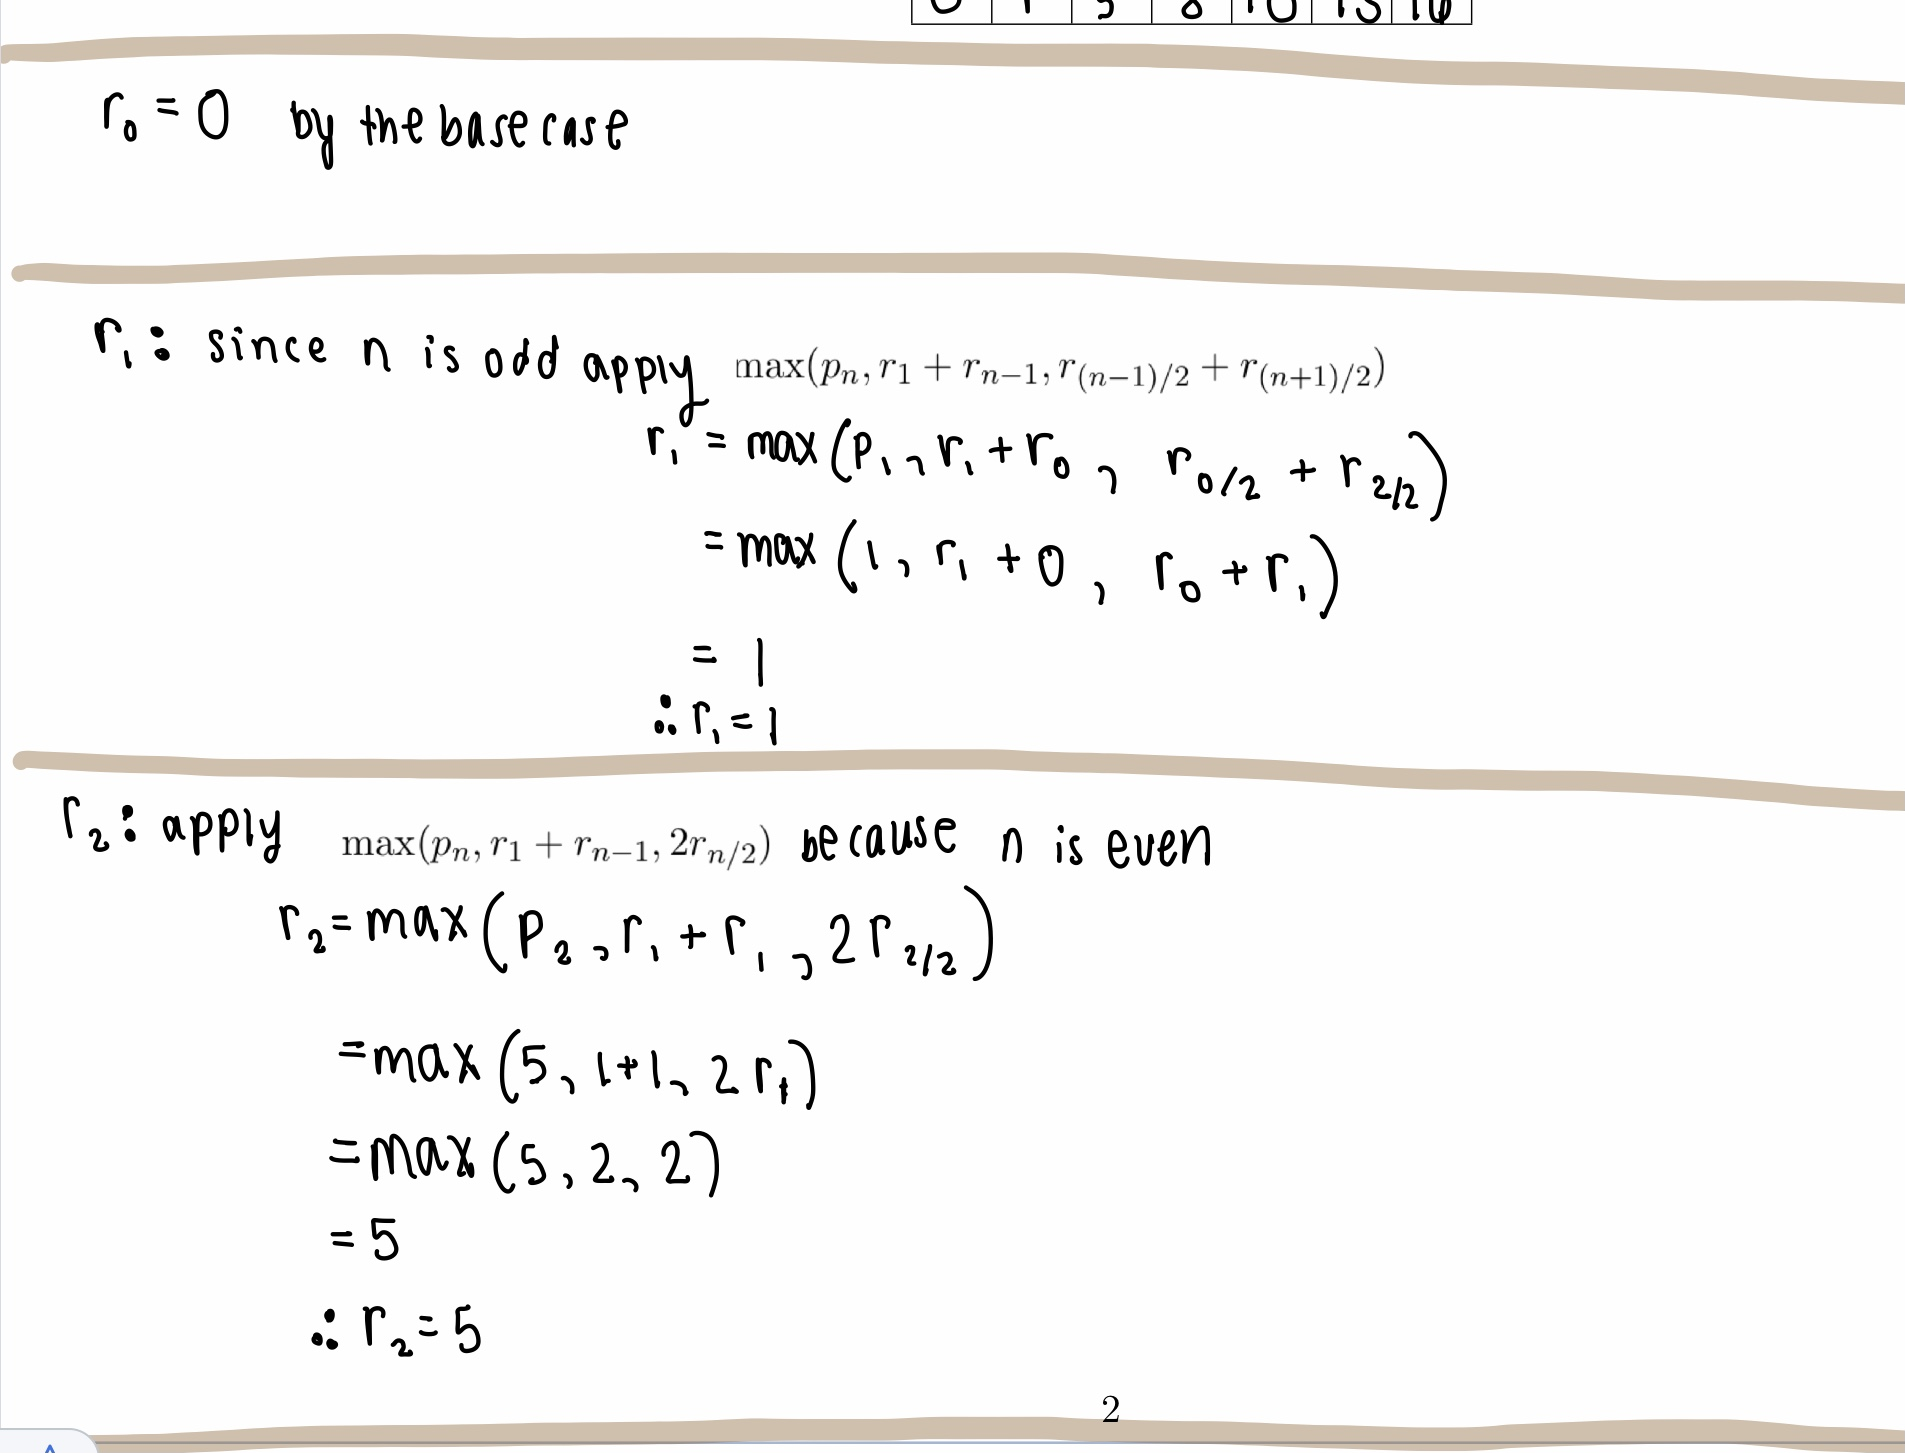
\includegraphics[width=0.8\textwidth]{q213}\\
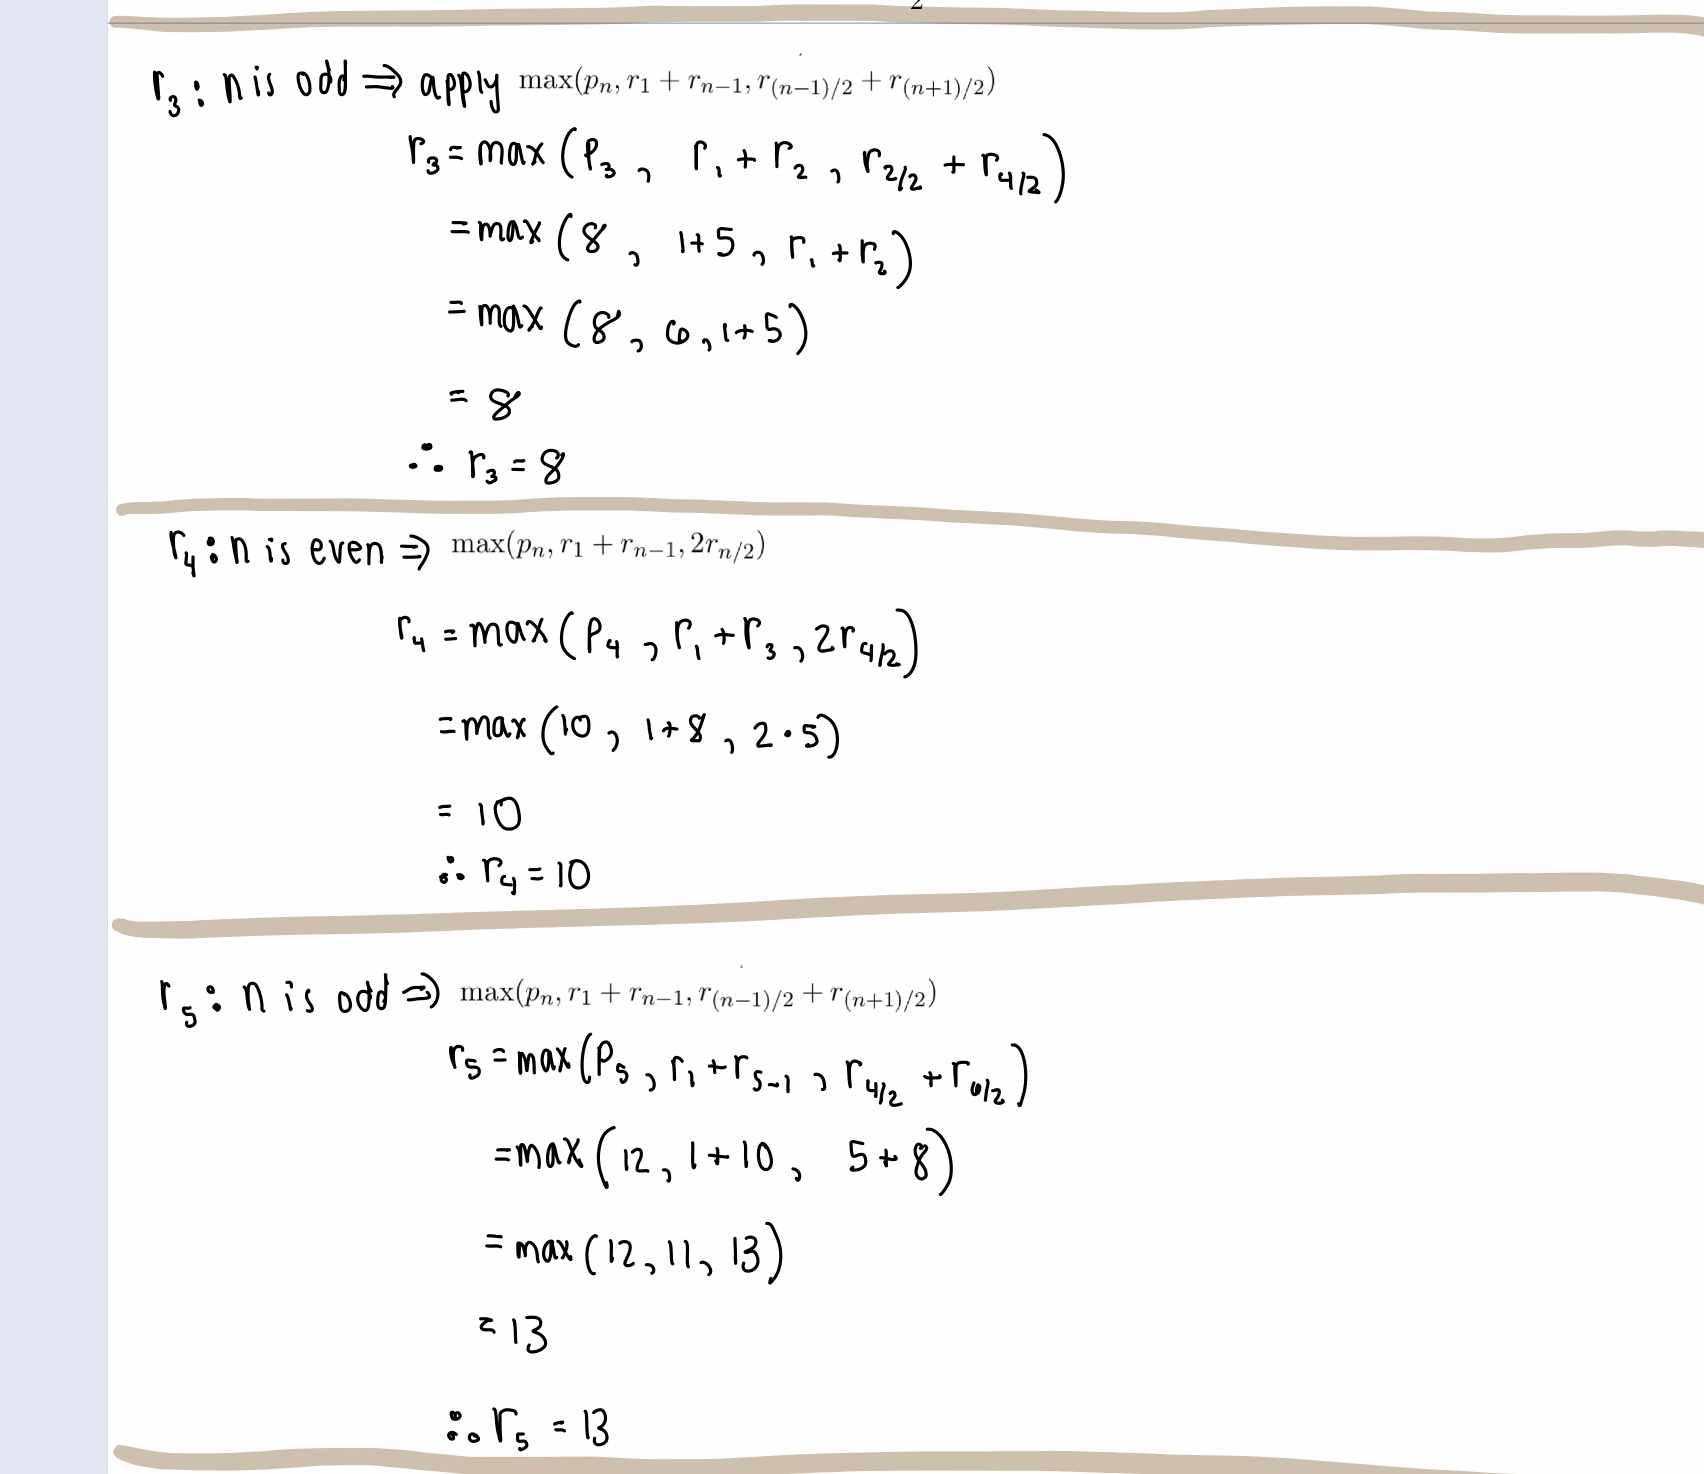
\includegraphics[width=0.8\textwidth]{q212}\\
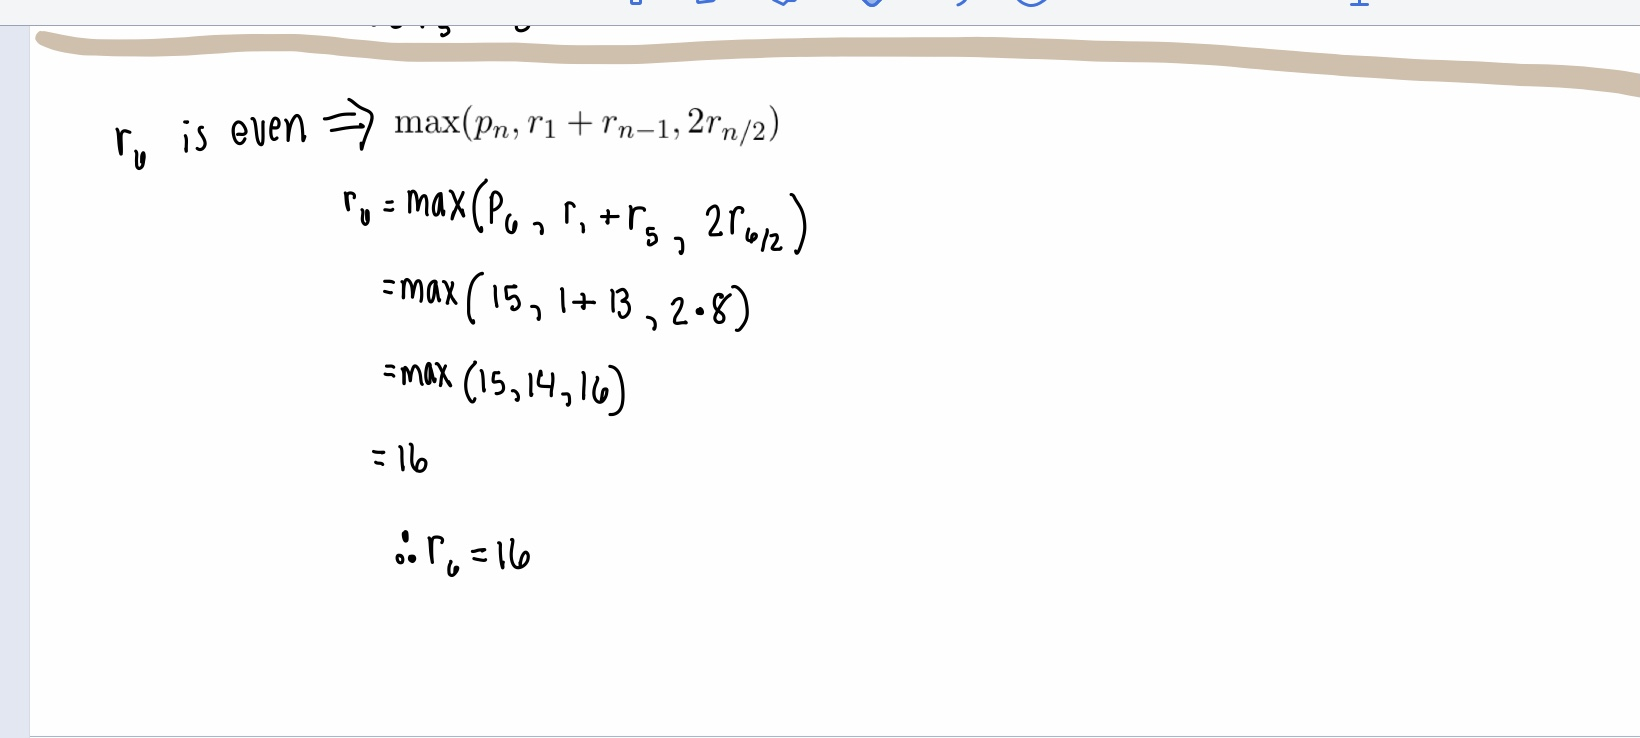
\includegraphics[width=0.7\textwidth]{q211}
\end{proof}

%%%%%%%%%%%%%%%%%%%%%%%%%%%%%%%%%%%%%%%%%%%%%%%%%%
\end{document} % NOTHING AFTER THIS LINE IS PART OF THE DOCUMENT



